% The quantized assembled matrix: upper blocks only (difference form), rows in SELL-C-sigma groups,
% one record of codes and scales per step, 16-bit column offsets, and the per-thread remainder.
% Drawn with C = 3 (16 in the code) on the mesh of the BSR diagram.
\documentclass[border=2pt]{standalone}
% Shared preamble of the format diagrams: colours of the paper's figures (paper_figures.py) and
% the drawing styles.  Each diagram is a standalone document built to a PDF of the text width.
\usepackage{amsmath,amssymb}
\usepackage{tikz}
\usetikzlibrary{arrows.meta,calc,decorations.pathreplacing,patterns,positioning}

\definecolor{cindex}{HTML}{BDBDBD}  % column indices, offsets, row pointers
\definecolor{cvalue}{HTML}{6E6E6E}  % floating-point values (BSR)
\definecolor{cpoint}{HTML}{1B9E77}  % quadrature-point store
\definecolor{celem}{HTML}{1F78B4}   % element matrix
\definecolor{cqbsr}{HTML}{A6761D}   % quantized BSR
\definecolor{cscale}{HTML}{E6AB02}  % scales
\definecolor{cmean}{HTML}{7570B3}   % f32 element mean

\tikzset{
  >={Stealth[length=4pt]},
  grid/.style={draw=black!45, line width=0.25pt},
  frame/.style={draw=black!70, line width=0.5pt},
  title/.style={font=\small\bfseries, anchor=west, inner sep=0pt},
  lab/.style={font=\footnotesize, inner sep=1pt},
  note/.style={font=\scriptsize, text=black!75, inner sep=1pt, execute at begin node={\hyphenpenalty=10000\exhyphenpenalty=10000}},
  num/.style={font=\tiny, inner sep=0pt},
  brace/.style={decorate, decoration={brace, amplitude=3pt, raise=1pt}, line width=0.4pt},
  arr/.style={->, line width=0.5pt, black!70},
  pad/.style={pattern=north east lines, pattern color=black!30},
}

% \cell{x}{y}{w}{h}{fill}: a filled rectangle with a thin outline, lower-left corner at (x,y).
\newcommand{\cell}[5]{\filldraw[fill=#5, grid] (#1,#2) rectangle ++(#3,#4);}
% \blk{x}{y}{s}{fill}: a 3x3 block of side s with its 3x3 entry grid.
\newcommand{\blk}[4]{%
  \filldraw[fill=#4, grid] (#1,#2) rectangle ++(#3,#3);
  \draw[draw=white, line width=0.25pt] (#1,#2) ++(#3/3,0) -- ++(0,#3) ++(#3/3,0) -- ++(0,-#3);
  \draw[draw=white, line width=0.25pt] (#1,#2) ++(0,#3/3) -- ++(#3,0) ++(0,#3/3) -- ++(-#3,0);
  \draw[grid] (#1,#2) rectangle ++(#3,#3);}
% \vthree{x}{y}{fill}: a 3-vector (one node's components) as three small cells, left end at (x,y).
\newcommand{\vthree}[3]{\foreach \k in {0,1,2} \filldraw[fill=#3, grid] (#1+\k*0.14,#2) rectangle ++(0.14,0.14);}
% \op{x}{y}{symbol}: an operation in a small circle.
\newcommand{\op}[3]{\node[circle, draw=black!70, line width=0.4pt, inner sep=0.5pt, minimum size=9pt, font=\tiny] at (#1,#2) {#3};}

\begin{document}
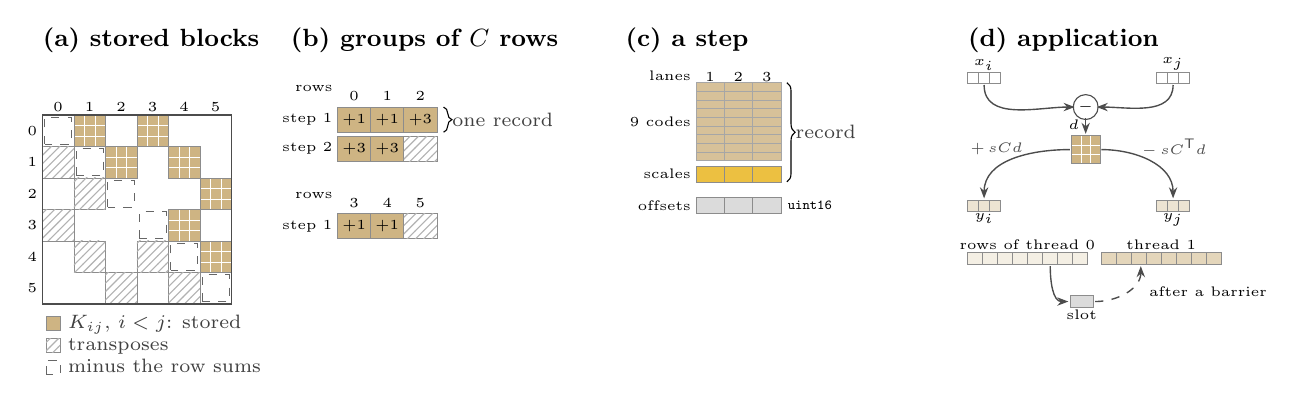
\begin{tikzpicture}
  % ---------------------------------------------------------------- (a) what is stored
  \def\s{0.4}
  \node[title] at (0, 3.35) {(a) stored blocks};
  \foreach \i/\cols in {0/{0,1,3}, 1/{0,1,2,4}, 2/{1,2,5}, 3/{0,3,4}, 4/{1,3,4,5}, 5/{2,4,5}} {
    \foreach \j in \cols {
      \pgfmathsetmacro{\x}{\j*\s}\pgfmathsetmacro{\y}{(5-\i)*\s}
      \ifnum\j>\i \blk{\x}{\y}{\s}{cqbsr!55}\fi
      \ifnum\j<\i \filldraw[fill=white, grid] (\x,\y) rectangle ++(\s,\s); \fill[pad] (\x,\y) rectangle ++(\s,\s); \fi
      \ifnum\j=\i \draw[grid, dashed, draw=black!60] (\x+0.03,\y+0.03) rectangle ++(\s-0.06,\s-0.06); \fi
    }
    \node[num, anchor=east] at (-0.06, {(5-\i)*\s+\s/2}) {$\i$};
    \node[num, anchor=south] at ({\i*\s+\s/2}, {6*\s+0.04}) {$\i$};
  }
  \draw[frame] (0,0) rectangle (6*\s, 6*\s);
  \node[note, anchor=north west, align=left] at (0, -0.1)
    {\tikz[baseline=0.2ex]\filldraw[fill=cqbsr!55, grid] (0,0) rectangle (0.18,0.18); $K_{ij}$, $i<j$: stored\\
     \tikz[baseline=0.2ex]{\filldraw[fill=white, grid] (0,0) rectangle (0.18,0.18); \fill[pad] (0,0) rectangle (0.18,0.18);} transposes\\
     \tikz[baseline=0.2ex]\draw[grid, dashed, draw=black!60] (0,0) rectangle (0.18,0.18); minus the row sums};

  % ---------------------------------------------------------------- (b) SELL-C-sigma groups
  \begin{scope}[shift={(3.75,0)}]
    \def\w{0.42}\def\h{0.32}
    \node[title] at (-0.6, 3.35) {(b) groups of $C$ rows};
    % group 1: rows 0, 1, 2, two steps; group 2: rows 3, 4, 5, one step.  Cells show j - i.
    \foreach \gy/\rows/\steps in {2.55/{0,1,2}/{{+1,+1,+3},{+3,+3,}}, 1.2/{3,4,5}/{{+1,+1,}}} {
      \foreach \r [count=\lane from 0] in \rows \node[num, anchor=south] at ({(\lane+0.5)*\w}, \gy+0.02) {$\r$};
      \foreach \offs [count=\st from 0] in \steps {
        \foreach \o [count=\lane from 0] in \offs {
          \pgfmathsetmacro{\x}{\lane*\w}\pgfmathsetmacro{\y}{\gy-(\st+1)*(\h+0.05)}
          \ifx\o\empty
            \filldraw[fill=white, grid] (\x,\y) rectangle ++(\w,\h); \fill[pad] (\x,\y) rectangle ++(\w,\h);
          \else
            \cell{\x}{\y}{\w}{\h}{cqbsr!55}
            \node[num] at (\x+\w/2, \y+\h/2) {$\o$};
          \fi
        }
      }
    }
    \node[num, anchor=east] at (-0.06, 2.55+0.18) {rows};
    \node[num, anchor=east] at (-0.06, 2.55-0.37+0.16) {step 1};
    \node[num, anchor=east] at (-0.06, 2.55-0.74+0.16) {step 2};
    \node[num, anchor=east] at (-0.06, 1.2+0.18) {rows};
    \node[num, anchor=east] at (-0.06, 1.2-0.37+0.16) {step 1};
    \draw[brace] (3*\w+0.05, 2.55-0.05) -- (3*\w+0.05, 2.55-0.37) node[midway, right=3pt, note] {one record};
  \end{scope}

  % ---------------------------------------------------------------- (c) one record
  \begin{scope}[shift={(8.3,0)}]
    \def\w{0.36}\def\rh{0.11}
    \node[title] at (-0.9, 3.35) {(c) a step};
    \foreach \lane in {1,2,3} \node[num, anchor=south] at ({(\lane-0.5)*\w}, 2.82) {$\lane$};
    \node[num, anchor=east] at (-0.06, 2.9) {lanes};
    \foreach \e in {0,...,8} \foreach \lane in {0,1,2}
      \filldraw[fill=cqbsr!45, draw=black!35, line width=0.15pt] (\lane*\w, {1.82+(8-\e)*\rh}) rectangle ++(\w,\rh);
    \node[num, anchor=east, align=right] at (-0.06, 2.32) {$9$ codes};
    \foreach \lane in {0,1,2} {\cell{\lane*\w}{1.55}{\w}{0.2}{cscale!75}}
    \node[num, anchor=east] at (-0.06, 1.65) {scales};
    \foreach \lane in {0,1,2} {\cell{\lane*\w}{1.15}{\w}{0.2}{cindex!55}}
    \node[num, anchor=east] at (-0.06, 1.25) {offsets};
    \draw[brace] (3*\w+0.04, 2.81) -- (3*\w+0.04, 1.55) node[midway, right=3pt, note, align=left] {record};
    \node[num, anchor=west] at (3*\w+0.08, 1.25) {\texttt{uint16}};
  \end{scope}

  % ---------------------------------------------------------------- (d) the application
  \begin{scope}[shift={(11.75,0)}]
    \node[title] at (0, 3.35) {(d) application};
    % one stored block K_ij, i < j
    \vthree{0.0}{2.8}{white} \node[num, anchor=south] at (0.21, 2.96) {$x_i$};
    \vthree{2.4}{2.8}{white} \node[num, anchor=south] at (2.61, 2.96) {$x_j$};
    \op{1.5}{2.5}{$-$}
    \draw[arr] (0.21, 2.78) to[out=-90, in=180] (1.36, 2.5);
    \draw[arr] (2.61, 2.78) to[out=-90, in=0] (1.64, 2.5);
    \draw[arr] (1.5, 2.36) -- (1.5, 2.16); \node[num, anchor=east] at (1.42, 2.27) {$d$};
    \blk{1.32}{1.78}{0.36}{cqbsr!55}
    \vthree{0.0}{1.18}{cqbsr!20} \node[num, anchor=north] at (0.21, 1.16) {$y_i$};
    \vthree{2.4}{1.18}{cqbsr!20} \node[num, anchor=north] at (2.61, 1.16) {$y_j$};
    \draw[arr] (1.3, 1.96) to[out=180, in=90] node[num, above left, pos=0.4] {$+\,sCd$} (0.21, 1.34);
    \draw[arr] (1.7, 1.96) to[out=0, in=90] node[num, above right, pos=0.4] {$-\,sC^{\mathsf T}d$} (2.61, 1.34);
    % threads: updates of another thread's rows go through slots
    \foreach \k in {0,...,7} {\cell{\k*0.19}{0.5}{0.19}{0.16}{cqbsr!12}}
    \foreach \k in {0,...,7} {\cell{1.7+\k*0.19}{0.5}{0.19}{0.16}{cqbsr!30}}
    \node[num, anchor=south] at (0.76, 0.68) {rows of thread $0$};
    \node[num, anchor=south] at (2.46, 0.68) {thread $1$};
    \cell{1.3}{-0.05}{0.3}{0.16}{cindex!55}
    \node[num, anchor=north] at (1.45, -0.07) {slot};
    \draw[arr] (1.05, 0.48) to[out=-90, in=180] (1.28, 0.03);
    \draw[arr, dashed] (1.62, 0.03) to[out=0, in=-90] (2.2, 0.48);
    \node[num, anchor=west] at (2.3, 0.15) {after a barrier};
  \end{scope}
\end{tikzpicture}
\end{document}
